\documentclass[11pt, a4paper]{article}
\usepackage[UKenglish]{babel}
\usepackage[bibstyle=ieee, dashed=false, sorting=nty]{biblatex}
\usepackage[labelfont=bf]{caption}
\usepackage{csquotes}
\usepackage{fancyhdr}
\usepackage{float}
\usepackage{graphicx}
\usepackage[top=25mm, right=20mm, bottom=25mm, left=20mm]{geometry}
\usepackage[hidelinks]{hyperref}
\usepackage{microtype}
\usepackage{parskip}
\usepackage[small,compact]{titlesec}

\titlespacing*{\section}{0pt}{\baselineskip}{0.35\baselineskip}

\pagestyle{fancy}
\fancyhf{}
\fancyhead[L]{COM3504}
\fancyhead[C]{The Intelligent Web: Assignment}
\fancyhead[R]{Team: Gakki}
\fancyfoot[C]{\thepage}

\addbibresource{references.bib}

\begin{document}
\section{Introduction}
Progressive Web App (PWA) allows users to create and add comments to both events and user stories. 
Social media features such as `like', `follow', `interested', and `going' are integrated. Users 
are able to tag an event along with their stories, which will then appear in the event page. Users 
can create a story by taking a picture with their front or environment camera through the 
implementation of WebRTC or upload a picture locally. Each user story can receive likes and comments, 
for which the latter is implemented using Socket.IO \cite{week6, socketio}. Service worker was 
implemented to cache requests for offline usage. MongoDB is used to store and synchronise data 
between the client and server, while IndexedDB is used to store data loaded from MongoDB for offline 
usage. However, data stored in MongoDB can only be retrieved when user is online. The search function 
(via location) was implemented with Google Maps API, allowing auto complete for the location field 
and ensuring that it is a valid location. For security purposes, users can only login with their 
respective Google Account.

\section{Diagrams}
\begin{figure}[H]
  \begin{center}
    \begin{minipage}[b]{0.4\textwidth}
      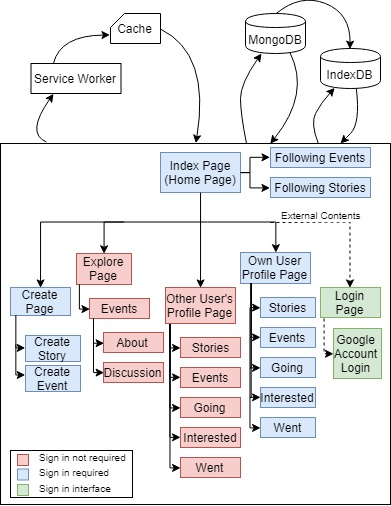
\includegraphics[width=6.5cm]{site_map.jpg}
      \caption{Demonstrates the flow of each web page in this PWA system along with the respective
      partial pages and external content pages.}
      \label{figure:site_map}
    \end{minipage}
    %
    \qquad
    \begin{minipage}[b]{0.4\textwidth}
      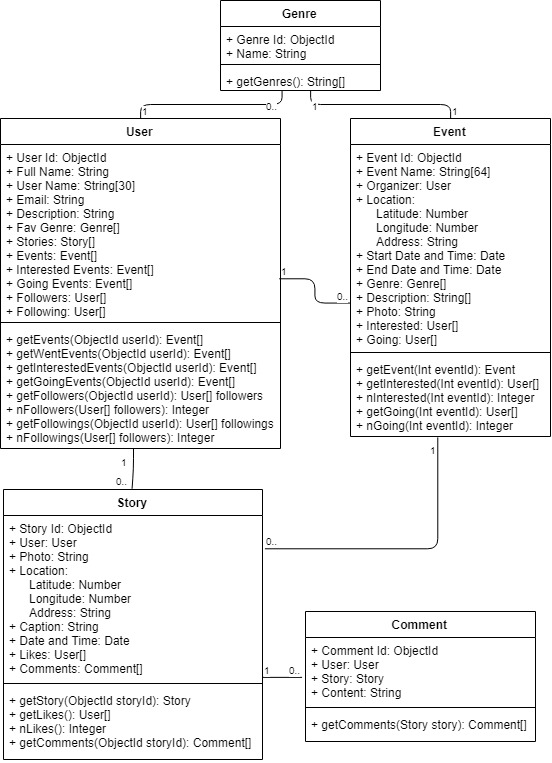
\includegraphics[width=6.5cm]{uml.jpg}
      \caption{Displays the structure of the database along with the types of content stored.}
      \label{figure:uml}
    \end{minipage}
  \end{center}
\end{figure}
\hyperref[figure:site_map]{\textbf{Figure 1}} and \hyperref[figure:uml]{\textbf{Figure 2}} are the
detailed description of the PWA system structure with \hyperref[figure:site_map]{\textbf{Figure 1}}
describing the front-end, data storage, caching and data retrieval, while
\hyperref[figure:uml]{\textbf{Figure 2}} demonstrates the database model in the database along with
the relationship between documents.

\section{Interface to Insert and Search Data via Forms}
\textbf{Challenges:} The search speed must be fast, and the results produced must be accurate with
respect to the query given. Users must be able to search for events, stories, and the profile of
other users. Basic text search will allow the user to input any text query and return the results
sorted by relevance. Advanced search will allow the user to search for events of a specific genre,
or find events between two different dates. Address searching in the event creation page is done by
using the Place Autocomplete of Google Maps API \cite{google_maps_api}.

\textbf{Solution:} FlexSearch.js \cite{flexsearch} is chosen for the basic text searching task due
to its fast, lightweight, and flexible features \cite{flexsearch_benchmarkk}. It allows multi-field
search and accepts multiple types of data format for its data index, hence it could be used with
both IndexedDB and MongoDB to provide searching functionality in both online and offline
environment. Advanced search are not implemented yet.

\textbf{Requirements:} Users should be able to search for events, stories, and user profiles while
online and offline. Users should be able to obtain results by querying partial part of the
information. The results returned should be sorted accoding to relevance.

\textbf{Limitations:} On every page load, the data has to be retrieved from IndexedDB to populate
the FlexSearch.js's search index. The performance loss might be negligible when the total data size
is small, but it may cause longer loading time when the total data exceeds certain size. Google Maps
API request could not be cached as it generates a random token for every request made, hence it will
not work offline.

\section{Interface to Search Data via Map (Yet to Implement)}
\textbf{Challenges} and \textbf{Solutions:} Not yet implemented.

\textbf{Requirements:} Allow users to search for events using a map in both online and offline
environment. Past events should not appear on the map. Future and ongoing events should be displayed
as custom markers on the map with different colour. Custom marker should pop up and displays the
event information when clicked.

\textbf{Limitations:} Caching the map tiles consumes more storage than other requests as map tiles
are stored as images. 

\section{PWA – Caching of the App Template Using a Web Worker}
\textbf{Challenges:} Fetching cross-domain response will result in an opaque response, which will
consume huge storage quota compared to normal responses \cite{opaque_workbox}. Sending a fallback
offline page response when user is offline and visit a page that does not exist in the cache.

\textbf{Solutions:} `Cache then network 'is implemented and modified accoding to The Offline
Cookbook \cite{offline_cookbook}.

\textbf{Requirements:} Users should be able to view a basic offline template with required data for
when offline. Users should be able to view previously loaded events and stories without the ability
to make any changes to the events, stories, or their profiles.

\textbf{Limitations:} Non-static files are not cached in the installation stage of the service
worker. Page that has never been visited before will not be cached. 

\section{PWA: Caching Data Using IndexedDB}
\textbf{Challenges:} Retrieving data from MongoDB and stored them into IndexedDB. Display page
content using data loaded from IndexedDB when no connection.

\textbf{Solution:} Retrieve the data from MongoDB using AJAX. Promise is used for both storing and
loading the data from IndexedDB.

\textbf{Requirements:} Events and user profile data must be stored locally for offline searching.
Users should be able to access the data retrieved from IndexedDB in offline.

\textbf{Limitations:} A known bug of IndexedDB storage usage increases with every $put()$ operation
\cite{leveldb_593, leveldb_603}. 

\section{NodeJS Server Including Non-Blocking Organisation of Multiple Dedicated Servers}
\textbf{Challenges:} Uses asynchronous functions to handle file upload, data retrieval from server,
or other functions call that requires time to complete. Errors might occurred during the execution
of asynchronous functions.

\textbf{Solution:} Uses the Promise and async/await features of JavaScript to handle both successful
and failed function operations. Keep the code nesting shallow to make code more maintainable and
readable.

\textbf{Requirements:} Able to use Promise to order the sequence of asynchronous processes. Able to
use callbacks to handle the successful and failure events of asynchronous functions.

\textbf{Limitations:} Single threaded mechanism, not suitable for CPU-intensive operations. Relies
heaviliy on callbacks, which might possible result in several callbacks nested within order
callbacks.

\section{MongoDB}
\textbf{Challenges:} Creating schemas that clearly defined the respective models. Verifying user
inputs when creating a new document. 

\textbf{Solution:} Uses mongoose's validation middleware \cite{validation} to define the values
allowed for an index.

\textbf{Requirements:} Data stored in MongoDB must be synchronised with IndexedDB when the client
has connection to the server.

\textbf{Limitations:} Less flexibility as it does not support joins between multiple documents.
Document size has a limit of 16MB, additional configurations required for storing large images.

\section{Quality of the Web Solution}
\textbf{Challenges:} Implementation of an authentication system. Social features such as user
profile, marking events as interested or going. Ensuring that the features implemented will work and
do not cause system failure.

\textbf{Solution:} Used passport-google-oauth20 \cite{passport_google} to implement the
authentication system. AJAX requests are used for a non-page reload form submittion. Exhaustively
testing the system to minimise the probability of bug occurrences.

\textbf{Requirements:} Users should be able to tag events in their stories, 'like' stories, 'follow'
other users, click 'interested' or 'going' on events. Events which users attended are recorded in
their profile. Users require a Google Account to login for security purposes.

\textbf{Limitations:} Users without a Google Account could not sign in into the system and enjoy
personalised content. User accounts are all public, hence users should be careful when sharing
personal

\section{Conclusions (To date of first submission)}
This assignment highlights the importance of caching and the importance of usability both during
online and offline. It taught us to consider other implementations to improve user experience and
web security. This assignment exposed us to multiple tools ( Google Maps API for address searching,
WebRTC for photo capturing, etc.) while allowing us to implement the basic knowledge of web building
at a higher level through the use of promises, service workers and memory caching.

\section{Division of Work (To date of first submission)}
The workload was divided equally. The solution was designed jointly and then each member lead the
implementation of one specific part of the code. \textbf{Zer Jun Eng} lead the implementation of all
PWA caching, MongoDB, and front-end implementation. \textbf{Lim Jia Mei Grace} implementation of
WebRTC, assisted in the construction of MongoDB database and front-end implementation.

\section{Extra Information}
With \textbf{mongod} service started, run \textbf{npm run initdb} to populate the database with
initial data.

\printbibliography

\end{document}
